%% CHANGE THIS ACCORDINGLY:
\newcommand{\authorFullName}{Ömer Faruk Deniz, Özdeniz Dolu}
\newcommand{\authorSchoolNumber}{2016400003, 2015400009}
%% AND NAME THE PROJECT UCO-surname-firstname-STAT-CS-YEAR (with or without dashes)

\newcommand{\courseName}{CMPE344 Final Project III Report}

\documentclass[12pt, oneside]{report}
\usepackage[margin=0.85in]{geometry}
\linespread{1}
\usepackage{xcolor}
\usepackage[colorlinks=false, linkbordercolor=white, citebordercolor=white, 
    filebordercolor=white, urlbordercolor=white]{hyperref}
    
\usepackage{graphicx}
\usepackage[utf8]{inputenc}
\usepackage[T1]{fontenc}
\usepackage[english]{babel}

\usepackage{fancyhdr}
\pagestyle{fancy}
\renewcommand{\headrulewidth}{0.4pt}
\fancyhead{}
\fancyhead[L]{\courseName\ -- Assignment}
\fancyhead[R]{\authorFullName}
\fancyfoot{}
\fancyfoot[C]{\thepage}

\usepackage{titlesec}
\titlespacing{\chapter}{0pt}{*4}{*2.5}

\titleformat{\chapter}{\normalfont\huge\bf}{\thechapter}{20pt}{\huge\bf}


% definition of an environment
\usepackage{listings}
\definecolor{deepblue}{rgb}{0,0,0.5}
\definecolor{deepred}{rgb}{0.6,0,0}
\definecolor{deepgreen}{rgb}{0,0.5,0}
\definecolor{burntsienna}{rgb}{0.91, 0.45, 0.32}

\lstset{
language=Python,
basicstyle=\ttm,
morekeywords={self},              % Add keywords here
keywordstyle=\ttb\color{deepblue},
commentstyle=\ttb\color{burntsienna},
emph={MyClass,__init__},          % Custom highlighting
emphstyle=\ttb\color{deepred},    % Custom highlighting style
stringstyle=\color{deepgreen},
frame=tb,                         % Any extra options here
showstringspaces=false,
numbers=left,
breaklines=true
}

\begin{document}
\begin{titlepage}
    \begin{center}
        \vspace*{1cm}
        
        \Huge
          \textbf{\courseName}
        
        \vspace{0.5cm}
        \LARGE
        
        \vspace{1.5cm}
        
        \textbf{\authorFullName}
        
        \vspace{1 cm}
        \authorSchoolNumber
   		  \vspace{1.5cm}
       
        \vfill
        
        
        \vspace{0.8cm}
          \Large
        Computer Engineering Department\\
        Boğaziçi University\\
        \vspace{0.5cm}
       \today{\year{}}
    \end{center}
\end{titlepage}
\tableofcontents
\addtocontents{toc}{~\hfill\textbf{Page}\par}
\chapter{Introduction}
\section{Problem Description}
In this project, we are expected to create a RISC-V pipelined datapath simulator on a high level programming language. Simulation is expected to implement hazard control and forwarding units as discussed throughout the lectures and in the course textbook. Simulation is also expected to keep data on CPI, total clock cycles, total number of stalls, stalls caused by instructions and prepare an output report on the execution using that data. Figure \ref{fig:datapath} is the diagram for the pipelined datapath structure taken from the course textbook. The simulator is also expected to simulate the instructions and, or, sub, add, beq, sd and ld. \\

\href{https://drive.google.com/drive/folders/104gLuhNgoEN1hMbGKwAH2UXVvRCwPsN0}{\color{blue}{GOOGLE DRIVE LINK FOR THE CODE}}
\begin{figure}
    \centering
    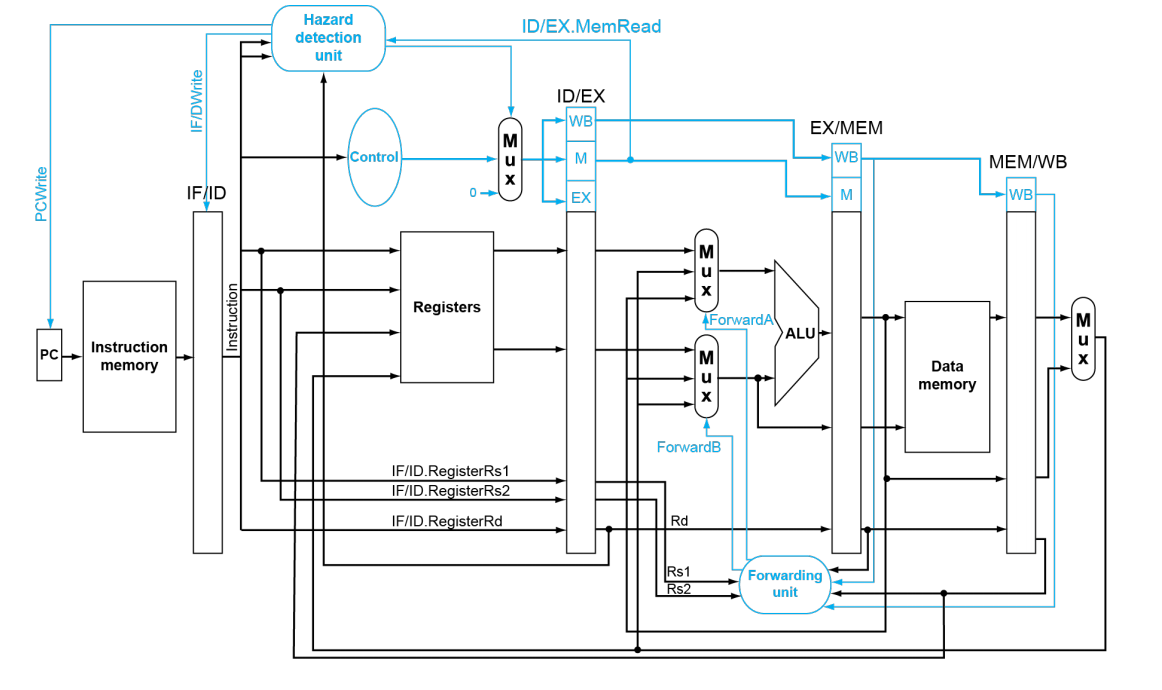
\includegraphics[scale=0.5]{1.png}
    \caption{Pipelined datapath diagram taken from course textbook}
    \label{fig:datapath}
\end{figure}

\section{Our Approach}
We have decided to write this simulator in the programming language Python. We aimed create a simulator structure that is strongly correlated with both the data and logical structure of the datapath. Simulator program, via a console argument, takes a plain text file that contains assembly code and some data initialization and fill the code in its virtual memory. Our simulator can run add. sub, and, or, beq, ld and sd instructions. Our simulator has variables for all the registers of RISC-V ISA and also for registers like ID/EX etc. We used the standard data structures of Python such as dictionaries and lists to simulate registers and memory. And to simulate the execution, we have defined methods for each phase of the datapath that are continuously executed one by one until the program counter reaches the end of the code. Those methods(for example a method for simulating the ID phase), during their execution, update the related registers according to their function. During the execution, simulator keeps all the related statistics to create a final report.


 % inputs file with main text
\chapter{Implementation and Modules}
\section{Input Format}
Simulator expects a path to a plain text file given as a first argument when running the code(see Chapter 3 for more details on running the simulator). Following segment is an example program.txt file.
\vspace{0.5 cm}

\begin{lstlisting}
x1=7
x2=18
m[5]=5
---
add x5,x1,x5
sub x1,x3,x2
ld x1,0(x5)
beq x1, x3, equal
equal:
add x6, x7, x8
\end{lstlisting}
\vspace{0.5 cm}

\noindent In our input format, lines that come before the --- separator line(line 4 in the above segment) are used for initializing the registers and memory of the simulator. This allows us to start the simulation in a more flexible set of states as by default all the memory and the registers are initialized at 0. Line 3 is a format for initalizing the memory. (addresses start at 0 and we are assuming double word addressing.)
\\

\noindent The lines that come after the --- separator line is the assembly code. Simulator can only process the instructions and, or, add, sub, beq, ld and sd. We are checking for excess whitespaces or similar formatting problems but still it is best to comply with the format shown in above segment.

\section{Modules}
\subsection{Simulator Class (simulator.py)}
\subsubsection{Constructor}
We have created a class for the simulation that keeps all the relevant data in the memory. Following code segment contains its constructor method. As can be seen in the first lines of the constructor method, registers and memory are kept as Python lists of corresponding sizes. \\

\noindent 
At the lines 24 to 30, one can see the initialization of the registers IF\_ID, ID\_EX, EX\_MEM, MEM\_WB. These registers are kept as Python dictionaries and they are the main channel of communication between the different stages of the pipelined execution. At every stage, the corresponding methods for that stage change the values that are written in these variables. They are intended to simulate the datapath circuitry in a one to one correspondance with the Figure \ref{fig:datapath}  
\\ 

\noindent This class also contains many more helper and/or main methods that we have omitted in this section due to inconvenience. They can be fully accessed through the code files.

\vspace{0.5 cm}
\begin{lstlisting}
class Simulator:
    def __init__(self, program_path):
        self.REGISTERS = [0] * 32 # REGISTER FILE
        self.MEMORY = [0] * 1000 # MEMORY
        self.PC = 0 # PROGRAM COUNTER
        self.CLOCK = 1 # CLOCK
        self.WORD_LEN = 4
        self.FLUSH = False

        self.FINISHED_INSTRUCTION_COUNT = 0
        init_lines, self.INSTRUCTION_NAMES, self.INSTRUCTION_MEMORY = get_program(program_path) # read program
        self.parse_inits(init_lines) # parse register and memory init commands
        
        self.NOP_INSTRUCTION = get_nop_instruction() # get nop instruction which has all fields 0
        self.NOP_CONTROL = get_nop_control() # all fields are 0
        self.ALL_STAGES_NOP = True # used to check if all stages are having NOP instructions

        self.stalls = {} # dictinary that holds instruction name and their stall counts
        self.STALL_OCCURRED = False # flag to check stall occurred in the current clock

        self.INSTRUCTIONS_IN_PIPELINE = ['NOP'] * 5 # name of instructions in the pipeline, used only for reporting purposes

        # fields of the stage registers and their initial values for NOP instructions
        self.IF_ID = {"PC": 0, "instruction": self.NOP_INSTRUCTION}
        self.ID_EX = {"PC": 0, "rs1_data": 0, "rs2_data": 0, 
            "imm_gen_offset": 0, "funct_for_alu_control": "0000", "rd": 0, 
            "control": self.NOP_CONTROL, "rs1": None, "rs2": None}
        self.EX_MEM = {"PC_plus_OFFSET": 0, "ALU_zero": 0, "ALU_result": 0, "rs1_data": 0, "rd": None,
            "control": self.NOP_CONTROL}
        self.MEM_WB = {"read_from_memory": 0, "ALU_result": 0, "rd": None, "control": self.NOP_CONTROL}
\end{lstlisting}


\subsubsection{run() method}
This is the main method that runs the simulation in a loop. Following is the code segment for the definition of this method from simulator.py. As can be seen in the line 6, while loop continues to execute the simulation until the PC reaches to end of the program or all of the stages have a NOP instructions in them. Former condition checks if the simulation is finished with all the instructions and the latter condition makes sure that no instruction is left in anywhere in the pipeline.
\\

\noindent In the lines 9 to 13, the simulation is happening as all the stages are run one by one, one after each other. All the stage outputs are in the format of their corresponding registers.
\\

\noindent The condition in the line 24 is to make sure the pipeline is flushed if a branching has occurred as if it is the case that branch condition is met, FLUSH variable will be set to True. We haven't implemented a branch prediction unit, therefore we need to flush every time. 
\vspace{0.5 cm}
\begin{lstlisting}
    def run(self):
        print(f"-----STATUS AT THE BEGINNING-----")
        print(*self.INSTRUCTIONS_IN_PIPELINE, sep=' | ')
        self.print_status()
        # while PC is valid and not all STAGES are filled with NOPs
        while(self.PC < len(self.INSTRUCTION_MEMORY) or not self.ALL_STAGES_NOP):
            PC_running = self.PC
            # run each stage separately before updating the stage registers
            self.run_WB()
            output_for_MEM_WB = self.run_MEM()
            output_for_EX_MEM = self.run_EX()
            output_for_ID_EX = self.run_ID()
            output_for_IF_ID = self.run_IF()

            # update the stage registers
            if not self.STALL_OCCURRED:
                self.IF_ID = output_for_IF_ID
            else: # self.IF_ID should be preserved if stall is occurred and instruction is fetched
                self.STALL_OCCURRED = False
            self.ID_EX = output_for_ID_EX
            self.EX_MEM = output_for_EX_MEM
            self.MEM_WB = output_for_MEM_WB
            # fill stage registers with NOP
            if self.FLUSH:
                self.PC = self.PC_plus_OFFSET
                self.IF_ID['instruction'] = self.NOP_INSTRUCTION
                self.ID_EX['control'] = self.NOP_CONTROL
                self.EX_MEM['control'] = self.NOP_CONTROL
                self.FLUSH = False


            print(f"-----STATUS AT THE END OF CLOCK = {self.CLOCK}-----")
            print(*self.INSTRUCTIONS_IN_PIPELINE, sep=' | ', end="")
            print(f" is run at PC = {PC_running}")
            self.print_status()
            #break
            self.CLOCK += 1
            # if all registers are full of control values of zero, namely NOPs update the flag
            if ((self.IF_ID['instruction'] == self.NOP_INSTRUCTION and self.ID_EX['control'] == self.EX_MEM['control']) and
                (self.EX_MEM['control'] == self.MEM_WB['control'] and self.MEM_WB['control'] == self.NOP_CONTROL)):
                self.ALL_STAGES_NOP = True
            else:
                self.ALL_STAGES_NOP = False
        self.CLOCK -= 1
        self.print_final_report()
\end{lstlisting}
\subsubsection{run\_IF() method}
This is the method that simulates the IF stage. Following is a code segment that contains its definition from the simulator.py file. The method simply fetches a new instruction from the instruction memory if the PC hasn't reached the end of the file. Members of the INSTRUCTION\_MEMORY contains the instructions as dictionaries with field such as rs1, rs2, rd etc. The return value of this function has the same structure as the IF\_ID register as it is going to be used to update that register.

\vspace{0.5 cm}
\begin{lstlisting}
    def run_IF(self):
        # if not all instructions are entered the pipeline
        if self.FLUSH:
            self.INSTRUCTIONS_IN_PIPELINE = ['NOP'] + self.INSTRUCTIONS_IN_PIPELINE[:-1]
            return {'PC':self.PC,'instruction': self.NOP_INSTRUCTION}
        if self.PC < len(self.INSTRUCTION_MEMORY) and not self.STALL_OCCURRED:
            new_instruction = self.INSTRUCTION_MEMORY[self.PC]
            self.INSTRUCTIONS_IN_PIPELINE = [self.INSTRUCTION_NAMES[self.PC // self.WORD_LEN]] + self.INSTRUCTIONS_IN_PIPELINE[:-1]
            PC = self.PC 
            self.PC += self.WORD_LEN
            return {'PC':PC, 'instruction': new_instruction, 'rs1': new_instruction['rs1'], 'rs2': new_instruction['rs2']}
        else: # add NOP to the pipeline
            if not self.STALL_OCCURRED:
                self.INSTRUCTIONS_IN_PIPELINE = ['NOP'] + self.INSTRUCTIONS_IN_PIPELINE[:-1]
            return {'PC':self.PC,'instruction': self.NOP_INSTRUCTION}
\end{lstlisting}

\subsubsection{run\_ID() method}
This is the method that simulates the ID stage. Following is a code segment that contains its definition from the simulator.py file. The method starts by accessing the instruction via the IF\_ID register. It uses some helper functions from the instruction.py file to get the related control values of that instruction. A hazard control unit for load use hazard is also implemented in this method as it can be seen at the line 18 and onward. This hazard can only be solved by adding a stall to the pipeline. The output format of this method has the same structure as ID\_EX register as it is going to be used to update that register.
\vspace{0.5 cm}
\begin{lstlisting}
    def run_ID(self):
        # read from stage registers
        instruction = self.IF_ID['instruction']
        PC = self.IF_ID['PC']

        # operate
        control = get_control_values(instruction) # calculate control
        imm_gen_offset = instruction['immed'] # sign extend the offset
        rs1 = instruction['rs1']
        rs2 = instruction['rs2']
        rs1_data = self.read_register(rs1)
        rs2_data = self.read_register(rs2)
        # will be used for setting ALU control in EX
        funct_for_alu_control = get_funct_for_alu_control(instruction)
        rd = instruction['rd']

        # check for hazard
        if self.ID_EX['control']['MemRead'] and ((self.ID_EX['rd'] == self.IF_ID['instruction']['rs1']) or (self.ID_EX['rd'] == self.IF_ID['instruction']['rs2'])):
            self.STALL_OCCURRED = True
            self.INSTRUCTIONS_IN_PIPELINE = [self.INSTRUCTIONS_IN_PIPELINE[0]] + ['NOP'] + self.INSTRUCTIONS_IN_PIPELINE[1:-1]
            stall_instruction = self.INSTRUCTIONS_IN_PIPELINE[2] # instruction in the ex stage causes the hazard
            # if already defined
            if stall_instruction in self.stalls:
                self.stalls[stall_instruction] += 1
            else:
                self.stalls[stall_instruction] = 1
            # return the output to be written to ID_EX
            return {"PC": 0, "rs1_data": 0, "rs2_data": 0, 
            "imm_gen_offset": 0, "funct_for_alu_control": "0000", "rd": 0, 
            "control": self.NOP_CONTROL, "rs1": None, "rs2": None}
        else:
            # return the output to be written to ID_EX
            return {"PC": PC, "rs1_data": rs1_data, "rs2_data": rs2_data, 
            "imm_gen_offset": imm_gen_offset, "funct_for_alu_control": funct_for_alu_control, "rd": rd, 
            "control": control, "rs1": rs1, "rs2": rs2}
\end{lstlisting}

\subsubsection{run\_EX() method}
This is the method that simulates the EX stage. Following is a code segment that contains its definition from the simulator.py file. The method starts by accessing the relevant data via the ID\_EX register. As can be seen starting from the line 16, method contains a forwarding unit to address EX and MEM hazards. After deciding on the hazard type by logical operations, method updates the corresponding forwarding unit bits. At the line 64 and onward it executes the EX stage by using the values that came from ID\_EX register or forwarded values if there are any. The output format of this method has the same structure as EX\_MEM register as it is going to be used to update that register.
\vspace{0.5 cm}
\begin{lstlisting}
    def run_EX(self):
        # read from stage registers
        control = self.ID_EX['control'] 
        PC = self.ID_EX['PC']
        rs1_data = self.ID_EX['rs1_data']
        rs2_data = self.ID_EX['rs2_data']
        imm_gen_offset = self.ID_EX['imm_gen_offset']
        funct_for_alu_control = self.ID_EX['funct_for_alu_control']
        rs1 = self.ID_EX['rs1']
        rs2 = self.ID_EX['rs2']
        rd = self.ID_EX['rd']

        # operate
        # forwarding unit
        # EX Hazard: pg 300 in the book
        ForwardA = "00"
        ForwardB = "00"
        if (self.EX_MEM['control']['RegWrite'] and (self.EX_MEM['rd'] != 0) and (self.EX_MEM['rd'] == self.ID_EX['rs1'])):
            ForwardA = "10"
        if (self.EX_MEM['control']['RegWrite'] and (self.EX_MEM['rd'] != 0) and (self.EX_MEM['rd'] == self.ID_EX['rs2'])):
            ForwardB = "10"

        # MEM Hazard: pg 301 in the book
        if (self.MEM_WB['control']['RegWrite'] and (self.MEM_WB['rd'] != 0) and not(self.EX_MEM['control']['RegWrite'] 
            and (self.EX_MEM['rd'] != 0) and (self.EX_MEM['rd'] == self.ID_EX['rs1'])) and (self.MEM_WB['rd'] == self.ID_EX['rs1'])):
            ForwardA = "01"
        if (self.MEM_WB['control']['RegWrite'] and (self.MEM_WB['rd'] != 0) and not(self.EX_MEM['control']['RegWrite'] 
            and (self.EX_MEM['rd'] != 0) and (self.EX_MEM['rd'] == self.ID_EX['rs2'])) and (self.MEM_WB['rd'] == self.ID_EX['rs2'])):
            ForwardB = "01"

        ALU_control = get_alu_control(str(control['ALUOp1'])+str(control['ALUOp0']), funct_for_alu_control)
        PC_plus_OFFSET = PC + 2 * imm_gen_offset # calculate PC offset
        ALU_result = None
        param1 = 0
        param2 = 0
        if ForwardA == "00":
            param1 = rs1_data
        elif ForwardA == "10":
            rs1_data = self.EX_MEM['ALU_result']
            param1 = rs1_data 
        elif ForwardA == "01":
            if self.MEM_WB['control']['RegWrite']:
                read_from_memory = self.MEM_WB['read_from_memory']
                ALU_result = self.MEM_WB['ALU_result']
                if self.MEM_WB['control']['MemToReg']: # ld: write the value at rs2+offset to rs1, else do not write to reg
                    param1 = read_from_memory
                else: # r-type: write the ALU_result to rd
                    param1 = ALU_result

        if ForwardB == "00":
            param2 = rs2_data
        elif ForwardB == "10":
            rs2_data = self.EX_MEM['ALU_result']
            param2 = rs2_data 
        elif ForwardB == "01":
            if self.MEM_WB['control']['RegWrite']:
                read_from_memory = self.MEM_WB['read_from_memory']
                ALU_result = self.MEM_WB['ALU_result']
                if self.MEM_WB['control']['MemToReg']: # ld: write the value at rs2+offset to rs1, else do not write to reg
                    param2 = read_from_memory
                else: # r-type: write the ALU_result to rd
                    param2 = ALU_result

        if control['ALUSrc'] == 0: # r-format or beq
            ALU_result = perform_ALU_operation(ALU_control, param1, param2)
        elif control['ALUSrc'] == 1: # ld, sd
            if control['MemWrite'] == 1: # sd: rs2_data+offset
                ALU_result = perform_ALU_operation(ALU_control, param2, imm_gen_offset)
            else: # ld: rs1_data+offset
                ALU_result = perform_ALU_operation(ALU_control, param1, imm_gen_offset)
        ALU_zero = ALU_result == 0

        # return the output to be written to EX_MEM
        return {"PC_plus_OFFSET": PC_plus_OFFSET, "ALU_zero": ALU_zero, 
            "ALU_result": ALU_result, "rs1_data": rs1_data, "rd": rd, "control": control}
\end{lstlisting}

\subsubsection{run\_MEM() method}
This is the method that simulates the MEM stage. Following is a code segment that contains its definition from the simulator.py file. The method starts by accessing the relevant data via the EX\_MEM register. It then proceeds to execute the MEM stage by checking if the instruction is a branch with branch condition met, sd with MemWrite set or ld with MemRead set. It creates a flush in the case of branch condition met and otherwise, it executes the corresponding memory operations and creates an output. The output format of this method has the same structure as MEM\_WB register as it is going to be used to update that register.
\vspace{0.5 cm}
\begin{lstlisting}
    def run_MEM(self):
        # read from stage registers
        control = self.EX_MEM['control'] # read control from previous stage
        PC_plus_OFFSET = self.EX_MEM['PC_plus_OFFSET']
        ALU_zero = self.EX_MEM['ALU_zero']
        ALU_result = self.EX_MEM['ALU_result']
        rs1_data = self.EX_MEM['rs1_data']
        rd = self.EX_MEM['rd']

        # operate
        if control['Branch'] and ALU_zero: # if a branch instruction and rs1_data-rs2_data == 0
            self.PC_plus_OFFSET = PC_plus_OFFSET
            # flush instructions in the IF, ID, EX when MEM is executing
            self.FLUSH = True
            self.INSTRUCTIONS_IN_PIPELINE = ['NOP', 'NOP'] + self.INSTRUCTIONS_IN_PIPELINE[2:]
            stall_instruction = self.INSTRUCTIONS_IN_PIPELINE[2]
            if stall_instruction in self.stalls:
                self.stalls[stall_instruction] += 3 # since flush adds two stalls to the pipeline
            else:
                self.stalls[stall_instruction] = 3
        if control['MemWrite']: # sd, will write to memory
            self.MEMORY[ALU_result] = rs1_data

        read_from_memory = None
        if control['MemRead']: # ld, will write to register file
            read_from_memory = self.MEMORY[ALU_result]
        
        # return the output to be written to MEM_WB
        return {"read_from_memory": read_from_memory, "ALU_result": ALU_result, "rd": rd, "control": control}
\end{lstlisting}

\subsubsection{run\_WB() method}
This is the method that simulates the WB stage. Following is a code segment that contains its definition from the simulator.py file. The method starts by accessing the relevant data via the MEM\_WB register. It then proceeds to execute WB stage by checking the values of RegWrite and MemToReg values to decide if the instruction is ld or an R-type instruction and writes to corresponding registers accordingly.
\vspace{0.5 cm}
\begin{lstlisting}
        def run_WB(self):
        # read from stage registers
        control = self.MEM_WB['control'] # read control from previous stage
        read_from_memory = self.MEM_WB['read_from_memory']
        ALU_result = self.MEM_WB['ALU_result']
        rd = self.MEM_WB['rd']
        # operate
        if control['RegWrite']:
            if control['MemToReg']: # ld: write the value at rs2+offset to rs1, else do not write to reg
                self.write_to_register(rd, read_from_memory)
            else: # r-type: write the ALU_result to rd
                self.write_to_register(rd, ALU_result)
        if control != self.NOP_CONTROL:
            self.FINISHED_INSTRUCTION_COUNT += 1
\end{lstlisting}

\subsection{Helper Functions (simulator.py)}
Simulator class contains many helper functions that are related to memory and register operations, stage executions and output printing. We omitted the code segments because they are long and redundant in many cases. Following is a list of helper functions in this file, briefly explained.

\begin{itemize}
    \item parse\_inits(self, init\_lines): This method parses and executes the register and memory initialialization lines of the input program file.
    \item write\_to\_register(self, index, value): This method writes the value to the register given as index, unless it is the register x0.
    \item read\_register(self, index): This method reads and returns the value of the given register.
    \item print\_status(self): This method prints the current values of registers and memory to the console but it omits the values that are equal to 0 for convenience.
    \item print\_final\_report(self): This method prints the final report on the simulation of the program. It is intended to be used when the execution is finished. It prints the values total number of clock cycles, CPI, total number of stalls, number of stalls caused by specific instructions.
    
    
\end{itemize}


\subsection{Helper Functions (instruction.py)}
This module contains many helper functions that are related to instructions, control values, ALU operations, parsing from the input program etc. We omitted the code segments because they are long and redundant in many cases. Following is a list of helper functions in this file, briefly explained.

\begin{itemize}
    \item get\_program(program\_path): This method parses the input program file and processes the instruction lines. Restructures all the instructions as an ordered list of dictionaries that contain fields such as rs1, rd, funct7 etc. Returns a list of those restructured instructions.
    \item perform\_ALU\_operation(ALU\_Control, param1, param2): This method takes a binary string ALU\_Control and decides on which operation to execute on parameters, Essentially simulates an ALU unit.    
    \item get\_alu\_control(ALU\_op, funct\_for\_alu\_control): This method returns the ALU\_Control binary string used by ALU unit by calculating it using its parameters.
    \item get\_nop\_instruction(): This method returns structured fields corresponding to a NOP instruction.
    \item get\_control\_values(instruction): This method returns a dictionary containing control values using the given instruction's opcode field.
    
    
\end{itemize}
\subsection{main.py}
This module is the runner program for the simulator. It processes the arguments given to the program and initializes the simulator accordingly.
\section{Output Format}
The simulator prints all its output to the console as formatted text. It can be printed into a file using terminal specific commands. The program outputs information about the status of the pipeline on every clock cycle and creates a final report containing statistics at the end of the execution. See Section 4 for sample executions and outputs. % inputs file with main text
\chapter{Execution \& Dependencies}
\noindent This simulator is tested and run on Windows 10 and Mac operating systems using Python 3.7. There are no other packages used other than those that come with Python 3 installation. Running the following terminal command on a folder that contains the code files and also a sample input program(described in Section 2.1) should be suffice to start the simulation.
\vspace{0.5 cm}

\begin{lstlisting}
python3 main.py program.txt
\end{lstlisting} % inputs file with main text
\chapter{Sample Simulations \& Outputs}
\noindent In this section, we investigate the simulator outputs on a number of different input programs.

\section{EX Hazard Example}
As we can see in output, no stalls have been introduced in dealing with this hazard as it is dealt by the forwarding unit. Total number of cycles is 6 as intended since the first instruction runs for 5 cycles and the second instruction tailing it add 1 more cycle to it. We see that final value for x2 is -6 and x19 is 3 which is correct. This example is taken from Chapter 4 Part 1 Slide 39.
\\

\noindent Input program:
\vspace{0.5 cm}
\begin{lstlisting}
x1=3
x3=9
---
add x19, x0, x1
sub x2, x19, x3
\end{lstlisting}
\vspace{0.5 cm}
Simulator output:
\vspace{0.5 cm}
\begin{lstlisting}
-----STATUS AT THE BEGINNING-----
NOP | NOP | NOP | NOP | NOP
x1: 3 x3: 9 
-----STATUS AT THE END OF CLOCK = 1-----
add x19, x0, x1 | NOP | NOP | NOP | NOP is run at PC = 0
x1: 3 x3: 9 
-----STATUS AT THE END OF CLOCK = 2-----
sub x2, x19, x3 | add x19, x0, x1 | NOP | NOP | NOP is run at PC = 4
x1: 3 x3: 9 
-----STATUS AT THE END OF CLOCK = 3-----
NOP | sub x2, x19, x3 | add x19, x0, x1 | NOP | NOP is run at PC = 8
x1: 3 x3: 9 
-----STATUS AT THE END OF CLOCK = 4-----
NOP | NOP | sub x2, x19, x3 | add x19, x0, x1 | NOP is run at PC = 8
x1: 3 x3: 9 
-----STATUS AT THE END OF CLOCK = 5-----
NOP | NOP | NOP | sub x2, x19, x3 | add x19, x0, x1 is run at PC = 8
x1: 3 x3: 9 x19: 3 
-----STATUS AT THE END OF CLOCK = 6-----
NOP | NOP | NOP | NOP | sub x2, x19, x3 is run at PC = 8
x1: 3 x2: -6 x3: 9 x19: 3 

-----FINAL REPORT-----
Total # of Clock Cycles: 6
Cycles per Instruction(CPI): 3
No stall occurred.
\end{lstlisting}

\section{Load-Use Hazard Example}
As we can see in the output, a stall has been inserted at the ID stage of load instruction as a load-use hazard has been detected in the run\_ID() method. This additional stall has increased the total number of cycles to 7 which makes the CPI 3.5. As we can see the final values of the x1 and x4, the instructions has been executed correctly as the results are as expected from the program. This example is taken from Chapter 4 Part 1 Slide 41.
\\

\noindent Input program:
\vspace{0.5 cm}
\begin{lstlisting}
x2=1
m[1]=10
x5=4
---
ld x1,0(x2)
sub x4,x1,x5

\end{lstlisting}
\vspace{0.5 cm}
Simulator output:
\vspace{0.5 cm}
\begin{lstlisting}
-----STATUS AT THE BEGINNING-----
NOP | NOP | NOP | NOP | NOP
x2: 1 x5: 4 m[1]: 10 
-----STATUS AT THE END OF CLOCK = 1-----
ld x1,0(x2) | NOP | NOP | NOP | NOP is run at PC = 0
x2: 1 x5: 4 m[1]: 10 
-----STATUS AT THE END OF CLOCK = 2-----
sub x4,x1,x5 | ld x1,0(x2) | NOP | NOP | NOP is run at PC = 4
x2: 1 x5: 4 m[1]: 10 
-----STATUS AT THE END OF CLOCK = 3-----
sub x4,x1,x5 | NOP | ld x1,0(x2) | NOP | NOP is run at PC = 8
x2: 1 x5: 4 m[1]: 10 
-----STATUS AT THE END OF CLOCK = 4-----
NOP | sub x4,x1,x5 | NOP | ld x1,0(x2) | NOP is run at PC = 8
x2: 1 x5: 4 m[1]: 10 
-----STATUS AT THE END OF CLOCK = 5-----
NOP | NOP | sub x4,x1,x5 | NOP | ld x1,0(x2) is run at PC = 8
x1: 10 x2: 1 x5: 4 m[1]: 10 
-----STATUS AT THE END OF CLOCK = 6-----
NOP | NOP | NOP | sub x4,x1,x5 | NOP is run at PC = 8
x1: 10 x2: 1 x5: 4 m[1]: 10 
-----STATUS AT THE END OF CLOCK = 7-----
NOP | NOP | NOP | NOP | sub x4,x1,x5 is run at PC = 8
x1: 10 x2: 1 x4: 6 x5: 4 m[1]: 10 

-----FINAL REPORT-----
Total # of Clock Cycles: 7
Cycles per Instruction(CPI): 3.5
Total # of Stalls: 1
Instructions and # of Stalls Caused: 
---> ld x1,0(x2): 1
\end{lstlisting}

\section{Multiple Hazards Example}
We see that in this input program there are multiple hazards. At lines 7 and 8 of the input program there is a load-use hazard, at lines 10 and 11 of the program there is another load-use hazard, at lines 8 and 9 there is an EX hazard and at lines 11 and 12 there is an EX hazard. Since EX hazards are dealt by the forwarding unit, no stalls have been introduced by them. We see that the two load-use hazards are dealt by introducing 2 different stalls. We see that the code correctly identified those stalls are resulted by the ld instructions and reported it. Looking at the final values of the registers and the memory, we see that all of the instructions have been executed correctly and the values are as expected from the program. This example is taken from Chapter 4 Part 1 Slide 42.
\\

\noindent Input program:
\vspace{0.5 cm}
\begin{lstlisting}
m[0]=2
m[8]=3
m[16]=23
x4=9
---
ld x1, 0(x0)
ld x2, 8(x0)
add x3, x1, x2
sd x3, 24(x0)
ld x4, 16(x0)
add x5, x1, x4
sd x5, 32(x0)
\end{lstlisting}
\vspace{0.5 cm}
Simulator output:
\vspace{0.5 cm}
\begin{lstlisting}
-----STATUS AT THE BEGINNING-----
NOP | NOP | NOP | NOP | NOP
x4: 9 m[0]: 2 m[8]: 3 m[16]: 23 
-----STATUS AT THE END OF CLOCK = 1-----
ld x1, 0(x0) | NOP | NOP | NOP | NOP is run at PC = 0
x4: 9 m[0]: 2 m[8]: 3 m[16]: 23 
-----STATUS AT THE END OF CLOCK = 2-----
ld x2, 8(x0) | ld x1, 0(x0) | NOP | NOP | NOP is run at PC = 4
x4: 9 m[0]: 2 m[8]: 3 m[16]: 23 
-----STATUS AT THE END OF CLOCK = 3-----
add x3, x1, x2 | ld x2, 8(x0) | ld x1, 0(x0) | NOP | NOP is run at PC = 8
x4: 9 m[0]: 2 m[8]: 3 m[16]: 23 
-----STATUS AT THE END OF CLOCK = 4-----
add x3, x1, x2 | NOP | ld x2, 8(x0) | ld x1, 0(x0) | NOP is run at PC = 12
x4: 9 m[0]: 2 m[8]: 3 m[16]: 23 
-----STATUS AT THE END OF CLOCK = 5-----
sd x3, 24(x0) | add x3, x1, x2 | NOP | ld x2, 8(x0) | ld x1, 0(x0) is run at PC = 12
x1: 2 x4: 9 m[0]: 2 m[8]: 3 m[16]: 23 
-----STATUS AT THE END OF CLOCK = 6-----
ld x4, 16(x0) | sd x3, 24(x0) | add x3, x1, x2 | NOP | ld x2, 8(x0) is run at PC = 16
x1: 2 x2: 3 x4: 9 m[0]: 2 m[8]: 3 m[16]: 23 
-----STATUS AT THE END OF CLOCK = 7-----
add x5, x1, x4 | ld x4, 16(x0) | sd x3, 24(x0) | add x3, x1, x2 | NOP is run at PC = 20
x1: 2 x2: 3 x4: 9 m[0]: 2 m[8]: 3 m[16]: 23 
-----STATUS AT THE END OF CLOCK = 8-----
add x5, x1, x4 | NOP | ld x4, 16(x0) | sd x3, 24(x0) | add x3, x1, x2 is run at PC = 24
x1: 2 x2: 3 x3: 5 x4: 9 m[0]: 2 m[8]: 3 m[16]: 23 m[24]: 5 
-----STATUS AT THE END OF CLOCK = 9-----
sd x5, 32(x0) | add x5, x1, x4 | NOP | ld x4, 16(x0) | sd x3, 24(x0) is run at PC = 24
x1: 2 x2: 3 x3: 5 x4: 9 m[0]: 2 m[8]: 3 m[16]: 23 m[24]: 5 
-----STATUS AT THE END OF CLOCK = 10-----
NOP | sd x5, 32(x0) | add x5, x1, x4 | NOP | ld x4, 16(x0) is run at PC = 28
x1: 2 x2: 3 x3: 5 x4: 23 m[0]: 2 m[8]: 3 m[16]: 23 m[24]: 5 
-----STATUS AT THE END OF CLOCK = 11-----
NOP | NOP | sd x5, 32(x0) | add x5, x1, x4 | NOP is run at PC = 28
x1: 2 x2: 3 x3: 5 x4: 23 m[0]: 2 m[8]: 3 m[16]: 23 m[24]: 5 
-----STATUS AT THE END OF CLOCK = 12-----
NOP | NOP | NOP | sd x5, 32(x0) | add x5, x1, x4 is run at PC = 28
x1: 2 x2: 3 x3: 5 x4: 23 x5: 25 m[0]: 2 m[8]: 3 m[16]: 23 m[24]: 5 m[32]: 25 
-----STATUS AT THE END OF CLOCK = 13-----
NOP | NOP | NOP | NOP | sd x5, 32(x0) is run at PC = 28
x1: 2 x2: 3 x3: 5 x4: 23 x5: 25 m[0]: 2 m[8]: 3 m[16]: 23 m[24]: 5 m[32]: 25 

-----FINAL REPORT-----
Total # of Clock Cycles: 13
Cycles per Instruction(CPI): 1.8571428571428572
Total # of Stalls: 2
Instructions and # of Stalls Caused: 
---> ld x2, 8(x0): 1
---> ld x4, 16(x0): 1
\end{lstlisting}

\section{Branching Example}
In this example we see a simple branching code. During execution of the first 2 instructions, we see that simulator detects that the branching condition is met at EX stage and therefore it flushes the remaining 3 instructions in the pipeline and jumps to the label lab1. This of course introduces new cycles due to the flushed stages, and as we see 3 stalls are counted at the end due to the flush. In the end we see that the execution is completed in 10 cycles. Since only 3 instructions are executed in total, the CPI value 3.33 is correct. Looking at the final values of the registers, we see that all of the values are correct and as expected from the code.
\\

\noindent Input program:
\vspace{0.5 cm}
\begin{lstlisting}
x1=7
x2=3
x3=4
---
add x6,x2,x2
beq x1,x1,lab1
add x7,x3,x3
add x10,x3,x3
lab2:
add x5,x1,x1
lab1:
add x11,x1,x1
\end{lstlisting}
\vspace{0.5 cm}
Simulator output:
\vspace{0.5 cm}
\begin{lstlisting}
-----STATUS AT THE BEGINNING-----
NOP | NOP | NOP | NOP | NOP
x1: 7 x2: 3 x3: 4 
-----STATUS AT THE END OF CLOCK = 1-----
add x6,x2,x2 | NOP | NOP | NOP | NOP is run at PC = 0
x1: 7 x2: 3 x3: 4 
-----STATUS AT THE END OF CLOCK = 2-----
beq x1,x1,lab1 | add x6,x2,x2 | NOP | NOP | NOP is run at PC = 4
x1: 7 x2: 3 x3: 4 
-----STATUS AT THE END OF CLOCK = 3-----
add x7,x3,x3 | beq x1,x1,lab1 | add x6,x2,x2 | NOP | NOP is run at PC = 8
x1: 7 x2: 3 x3: 4 
-----STATUS AT THE END OF CLOCK = 4-----
add x10,x3,x3 | add x7,x3,x3 | beq x1,x1,lab1 | add x6,x2,x2 | NOP is run at PC = 12
x1: 7 x2: 3 x3: 4 
-----STATUS AT THE END OF CLOCK = 5-----
NOP | NOP | NOP | beq x1,x1,lab1 | add x6,x2,x2 is run at PC = 16
x1: 7 x2: 3 x3: 4 x6: 6 
-----STATUS AT THE END OF CLOCK = 6-----
add x11,x1,x1 | NOP | NOP | NOP | beq x1,x1,lab1 is run at PC = 20
x1: 7 x2: 3 x3: 4 x6: 6 
-----STATUS AT THE END OF CLOCK = 7-----
NOP | add x11,x1,x1 | NOP | NOP | NOP is run at PC = 24
x1: 7 x2: 3 x3: 4 x6: 6 
-----STATUS AT THE END OF CLOCK = 8-----
NOP | NOP | add x11,x1,x1 | NOP | NOP is run at PC = 24
x1: 7 x2: 3 x3: 4 x6: 6 
-----STATUS AT THE END OF CLOCK = 9-----
NOP | NOP | NOP | add x11,x1,x1 | NOP is run at PC = 24
x1: 7 x2: 3 x3: 4 x6: 6 
-----STATUS AT THE END OF CLOCK = 10-----
NOP | NOP | NOP | NOP | add x11,x1,x1 is run at PC = 24
x1: 7 x2: 3 x3: 4 x6: 6 x11: 14 

-----FINAL REPORT-----
Total # of Clock Cycles: 10
Cycles per Instruction(CPI): 3.3333333333333335
Total # of Stalls: 3
Instructions and # of Stalls Caused: 
---> beq x1,x1,lab1: 3
\end{lstlisting}


\section{MEM Hazard Example}
This is a MEM hazard example. Since the forwarding unit is dealing with the MEM hazard, we see that no stalls are introduced. Therefore, the execution ends in 7 cycles as expected. We see that the final values of the registers are as expected from the correct execution. Which means that the forwarding unit has done its job properly.
\\

\noindent Input program:
\vspace{0.5 cm}
\begin{lstlisting}
x2=3
m[3]=7
x4=5
---
ld x1, 0(x2)
add x3,x2,x2
add x4, x1, x4
\end{lstlisting}
\vspace{0.5 cm}
Simulator output:
\vspace{0.5 cm}
\begin{lstlisting}
-----STATUS AT THE BEGINNING-----
NOP | NOP | NOP | NOP | NOP
x2: 3 x4: 5 m[3]: 7 
-----STATUS AT THE END OF CLOCK = 1-----
ld x1, 0(x2) | NOP | NOP | NOP | NOP is run at PC = 0
x2: 3 x4: 5 m[3]: 7 
-----STATUS AT THE END OF CLOCK = 2-----
add x3,x2,x2 | ld x1, 0(x2) | NOP | NOP | NOP is run at PC = 4
x2: 3 x4: 5 m[3]: 7 
-----STATUS AT THE END OF CLOCK = 3-----
add x4, x1, x4 | add x3,x2,x2 | ld x1, 0(x2) | NOP | NOP is run at PC = 8
x2: 3 x4: 5 m[3]: 7 
-----STATUS AT THE END OF CLOCK = 4-----
NOP | add x4, x1, x4 | add x3,x2,x2 | ld x1, 0(x2) | NOP is run at PC = 12
x2: 3 x4: 5 m[3]: 7 
-----STATUS AT THE END OF CLOCK = 5-----
NOP | NOP | add x4, x1, x4 | add x3,x2,x2 | ld x1, 0(x2) is run at PC = 12
x1: 7 x2: 3 x4: 5 m[3]: 7 
-----STATUS AT THE END OF CLOCK = 6-----
NOP | NOP | NOP | add x4, x1, x4 | add x3,x2,x2 is run at PC = 12
x1: 7 x2: 3 x3: 6 x4: 5 m[3]: 7 
-----STATUS AT THE END OF CLOCK = 7-----
NOP | NOP | NOP | NOP | add x4, x1, x4 is run at PC = 12
x1: 7 x2: 3 x3: 6 x4: 12 m[3]: 7 

-----FINAL REPORT-----
Total # of Clock Cycles: 7
Cycles per Instruction(CPI): 2.3333333333333335
No stall occurred.
\end{lstlisting}

\section{Double Data Hazard Example}
This is a double data hazard example. There is a MEM hazard between lines 5 and 7 and there is an EX hazard between the lines 6 and 7. Correct forwarding action is to give priority to the EX hazard and forward the ALU result from the line 6 to the line 7. We see in the output that indeed, forwarding unit of our simulator is correctly forwarding as the final values of the registers are correct and as expected. This example is taken from the Chapter 4 Part 2 Slide 30.
\\

\noindent Input program:
\vspace{0.5 cm}
\begin{lstlisting}
x2=2
x3=3
x4=4
---
add x1,x1,x2
add x1,x1,x3
add x1,x1,x4
\end{lstlisting}
\vspace{0.5 cm}
Simulator output:
\vspace{0.5 cm}
\begin{lstlisting}
-----STATUS AT THE BEGINNING-----
NOP | NOP | NOP | NOP | NOP
x2: 2 x3: 3 x4: 4 
-----STATUS AT THE END OF CLOCK = 1-----
add x1,x1,x2 | NOP | NOP | NOP | NOP is run at PC = 0
x2: 2 x3: 3 x4: 4 
-----STATUS AT THE END OF CLOCK = 2-----
add x1,x1,x3 | add x1,x1,x2 | NOP | NOP | NOP is run at PC = 4
x2: 2 x3: 3 x4: 4 
-----STATUS AT THE END OF CLOCK = 3-----
add x1,x1,x4 | add x1,x1,x3 | add x1,x1,x2 | NOP | NOP is run at PC = 8
x2: 2 x3: 3 x4: 4 
-----STATUS AT THE END OF CLOCK = 4-----
NOP | add x1,x1,x4 | add x1,x1,x3 | add x1,x1,x2 | NOP is run at PC = 12
x2: 2 x3: 3 x4: 4 
-----STATUS AT THE END OF CLOCK = 5-----
NOP | NOP | add x1,x1,x4 | add x1,x1,x3 | add x1,x1,x2 is run at PC = 12
x1: 2 x2: 2 x3: 3 x4: 4 
-----STATUS AT THE END OF CLOCK = 6-----
NOP | NOP | NOP | add x1,x1,x4 | add x1,x1,x3 is run at PC = 12
x1: 5 x2: 2 x3: 3 x4: 4 
-----STATUS AT THE END OF CLOCK = 7-----
NOP | NOP | NOP | NOP | add x1,x1,x4 is run at PC = 12
x1: 9 x2: 2 x3: 3 x4: 4 

-----FINAL REPORT-----
Total # of Clock Cycles: 7
Cycles per Instruction(CPI): 2.3333333333333335
No stall occurred.
\end{lstlisting}

 % inputs file with main text
\end{document}